\documentclass[10pt,letterpaper]{amspset}
\usepackage{fullpage}
\usepackage{gensymb}
\usepackage{graphicx}
\usepackage{tikz}
\usepackage{amsmath}
\usepackage{pgfplots}
\usepackage{amsthm}
\usepackage{amssymb}
\pgfplotsset{compat=1.17}
\graphicspath{ {./images/} }
\notag

% info for header block in upper right hand corner
\name{Brady Lamson}
\class{MATH 1120 SPRING 2021}
\assignment{Graphing Trig Functions Part 2}
\duedate{Feb 21st}
\begin{document}

\problemlist{Graphs of the Trigonometric Functions Part II:  

10.5: 29--31, 35, 36, 38--40, 44--51}

For exercises 29--31 show that the following functions are sinusoids by rewriting them in the forms $C(x) = A\cos(\omega x + \phi) + B$ and $S(x) = A\sin(\omega x + \phi) + B$ for $\omega > 0$ and $0 \leq \phi < 2\pi$.

\begin{problem}[29]
    $f(x) = 2\sqrt{3}\cos(x) - 2\sin(x)$ 
\end{problem}

\begin{solution}
    Before we can start the actual process of solving this problem it would be wise to state information we will be utilizing.
    
   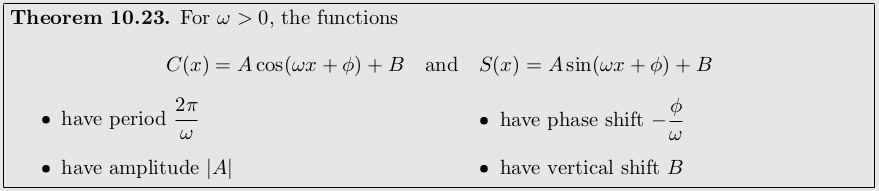
\includegraphics[width=6in,scale=1.0]{images/theorem_10.23.png}
   
   We're also going to need the sum formulas for both sine and cosine to solve this problem. 
   
    \begin{align}
        \sin (\alpha \pm \beta) = \sin(\alpha) \cos(\beta) \pm \cos(\alpha) \sin(\beta) \\
        \cos (\alpha \pm \beta) = \cos(\alpha) \cos(\beta) \mp \sin(\alpha) \sin(\beta)
    \end{align}
    
    This problem allows us to make some assumptions so let's list off our givens. We can assume that $B$ is 0 due to there being no vertical shift at the end of our function. I will also be assuming that $\omega = 1$ due to the structure of our function though this won't really be relevant due to how I will solve this.  
    
    \begin{align}
        B = 0 && \omega = 1 \\
        A = ? && \phi = ?
    \end{align}
    
    Okay, now we have the tools we need to work through this. The overall gameplan will be to take $C(x)$ and work it through the format of the expanded sum formulas. We will then substitute in values from $f(x)$. Doing this will allow us to solve for information we don't have, that being A and $\phi$. We will first start with the expanded formula of cosine. 

    \[ C(x) = A\cos(\omega x + \phi) + B \]
    
    What's useful about $C(x)$ is that with a little work it fits very nicely into the format of our sum formulas listed above. For this we will let $\omega x = \alpha$ and $\phi = \beta$. 
    
    \pagebreak 
    
    \begin{align}
        2\sqrt{3}\cos(x) - 2\sin(x) &= \cos(\alpha) \cos(\beta) \mp \sin(\alpha) \sin(\beta) \\
        2\sqrt{3}\cos(x) - 2\sin(x) &= A \cos(\omega x) \cos(\phi) + A \sin(\omega x) \sin(\phi) + B \\
        \intertext{Since we're dealing with multiplication here we can rewrite this as:}
        2\sqrt{3}\cos(x) - 2\sin(x) &= A \cos(\phi) \cos(\omega x) + A \sin(\phi) \sin(\omega x) + B \\
        \intertext{There's something else interesting here. We can equate the coefficients on either side of our equation. Doing so we can say the following:}
        2\sqrt{3}cos(x) &= A \cos(\phi) \cos(\omega x) \\
        2\sqrt{3} &= A \cos(\phi) \\
        2\sin(x) &= A \sin(\phi) \sin(\omega x) \\
        2\sin(x) &= A \sin(\phi) \\
        \intertext{We can actually use another identity now: the Pythagorean identity.}
        \cos^2(\phi) + \sin^2(\phi) &= 1 \\
        \intertext{Now, we can multiply this identity by $A^2$ and then substitute in our values.}
        A^2 \cos^2(\phi) + A^2 \sin^2(\phi) &= A^2 \\
        (2\sqrt{3})^2 + 2^2 &= A^2 \\
        12 + 4 &= A^2 \\
        \pm 4 &= A
    \end{align}

    Okay, that was a lot but we're finally getting somewhere here. We solved for A, now we can solve for $\phi$. The thing to keep in mind is that we have two values of A here, a positive and a negative value. The value we choose ends up not mattering which I will showcase later. To start though, I will choose positive 4. 
    \begin{align}
        2\sqrt{3} &= A \cos(\phi) && A \sin(\phi) = 2\sin(x) \\
        2\sqrt{3} &= 4 \cos(\phi) && 4 \sin(\phi) = 2\sin(x) \\
        \cos(\phi) &= \frac{2 \sqrt{3}}{4} && \sin(\phi) = \frac{1}{2} \\
        \cos(\phi) &= \frac{\sqrt{3}}{2}
    \end{align}

    This step is easy, we just need to find the values on the unit circle where each of these is true. 

    \[ \cos(\phi) = \frac{\sqrt{3}}{2} \text{  when  } \phi = \frac{\pi}{6} \text{  or  } \frac{11\pi}{6}\]
    \[ \sin(\phi) = \frac{1}{2} \text{  when  } \phi = \frac{\pi}{6} \text{  or  } \frac{5\pi}{6}\]

    So, it seems like $\phi = \frac{\pi}{6}$ is our culprit. Perfect. We're not done yet though! 

\pagebreak

    To be thorough let's go ahead and check $A = -4$ as well. I'll spare you the calculations, all we need to do is flip the signs. We get $\cos(\phi) = -\frac{\sqrt{3}}{2}$ and $\sin(\phi) = -\frac{1}{2}$. 
    
    \[ \cos(\phi) = -\frac{\sqrt{3}}{2} \text{  when  } \phi = \frac{5\pi}{6} \text{  or  } \frac{7\pi}{6}\]
    \[ \sin(\phi) = -\frac{1}{2} \text{  when  } \phi = \frac{11\pi}{6} \text{  or  } \frac{7\pi}{6}\]
    
    Our culprit now is $\phi = \frac{7\pi}{6}$. What's interesting here is that these are different values of $\phi$. Let's plot them and see what's going on. Before we can do that though, let's finish the first part of this problem and plug these values back into $C(x)$.
    
    \[ C(x) = 4 cos \left( x + \frac{\pi}{6} \right) \]
    \[ C(x) = -4 cos \left( x + \frac{7\pi}{6} \right) \]
    
    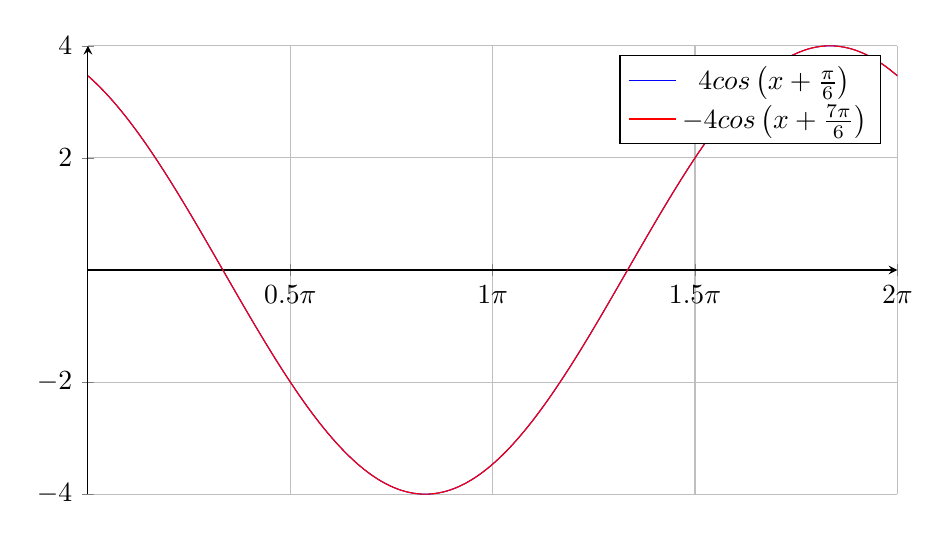
\begin{tikzpicture}
        \begin{axis}
            [
            grid=both,
            axis lines=middle,
            domain=0:2*pi,
            samples=200,
            no marks,
            xticklabels={-2$\pi$,-1.5$\pi$,...$\pi$,2$\pi$},
            xtick={-6.2832,-4.7124,...,6.2832},
            x post scale=1.5
            ]
            \addplot {4 * cos(deg(x + (pi / 6)};
            \addlegendentry{$4 cos \left( x + \frac{\pi}{6} \right)$};
            \addplot {-4 * cos(deg(x + ((7 * pi) / 6))};
            \addlegendentry{$-4 cos \left( x + \frac{7\pi}{6} \right)$};
        \end{axis}
    \end{tikzpicture}
    
    What we see here is that the two graphs overlap. They're equivalent functions. To describe what's going on the difference in phase shifts is, in a way, negated by the flip. As such both answers here are correct. Both ways of writing out $C(x)$ are equally valid!  
    
    So, I mentioned earlier that I simply assumed $\omega =1$ but that how I solved the problem made that irrelevant. Let's go through and solve for $\omega$ just to be positive. To do this we will simply substitute back in everything we know into our formula and solve!
    
    For the following, let $\alpha = \omega x$ and $\beta = \phi$ as always.
    \begin{align}
        A \cos(\omega x + \phi) &= 2\sqrt{3}\cos(x) - 2sin(x) \\
        A \cos(\omega x) \cos(\phi) \mp A \sin(\omega x) \sin(\phi) &= 2\sqrt{3}\cos(x) - 2sin(x) \\
        A \cos(\phi) \cos(\omega x) \mp A \sin(\phi) \sin(\omega x) &= 2\sqrt{3}\cos(x) - 2sin(x) \\
        4 \cos(\frac{11\pi}{6}) cos(\omega x) \mp 4 \sin(\frac{11\pi}{6}) \sin(\omega x) &= 2\sqrt{3}\cos(x) - 2sin(x) \\
        4 \left( \frac{\sqrt{3}}{2} \right) cos(\omega x) \mp 4 \left( - \frac{1}{2} \right) \sin(\omega x) &= 2\sqrt{3}\cos(x) - 2sin(x) \\
        2\sqrt{3} cos(\omega x) \mp -2 sin(\omega x) &= 2\sqrt{3}\cos(x) - 2sin(x) \\
        \intertext{Note: Due to the $-2sin(x)$ on the righthand side we know that the $\mp$ we have on the lefthand side will be a plus sign. They have to be inverted.}
        2\sqrt{3} cos(\omega x) + -2 sin(\omega x) &= 2\sqrt{3}\cos(x) - 2sin(x) \\
        2\sqrt{3} cos(\omega x) -2 sin(\omega x) &= 2\sqrt{3}\cos(x) - 2sin(x) \\
        \intertext{The left and righthand side are now identical!}
        \therefore \\
        \omega &= 1
    \end{align}
    
    Okay, so we're on the fourth page and I need to reassure you that we're almost there. All we need to do now is go back to the beginning and work through $S(x)$ in the same way. It'll be faster this time though! So, of course first we need to equate $f(x)$ with $S(x)$. Also recall that $\omega = 1$ and $B = 0$.
    
    \[ f(x) = 2\sqrt{3}cos(x) - 2sin(x)\]
    \[ S(x) = A \sin(\omega x + \phi) + B\]
    \[ sin(\alpha \pm \beta) = \sin(\alpha) \cos(\beta) \pm \cos(\alpha) \sin(\beta) \]
    We'll let $\alpha = \omega x$ amd $\beta = \phi$ just as last time.
    
    \begin{align}
        2\sqrt{3}cos(x) - 2sin(x) &= A \sin(\omega x - \phi) + B \\
        2\sqrt{3}cos(x) - 2sin(x) &= A \sin(\omega x) \cos(\phi) - A \cos(\omega x) sin(\phi) + B \\
        2\sqrt{3}cos(x) - 2sin(x) &= - A \cos(x) sin(\phi) + A \sin(x) \cos(\phi) + 0 \\
        2\sqrt{3}cos(x) - 2sin(x) &= - A sin(\phi) \cos(x) + A \cos(\phi) \sin(x) \\
        \intertext{Alright, so now we equate the coefficients again. You know how it goes.}
        2\sqrt{3}cos(x) &= - A \sin(\phi) \cos(x)  && 2sin(x) = A \cos(\phi) \sin(x) \\
        -2\sqrt{3} &= A\sin(\phi) && 2 = A\cos(\phi) \\
    \end{align}
        
        Time to do the Pythagorean identity again just to be certain of our A value.
    \begin{align}
        \cos^2(\phi) + \sin^2(\phi) &= 1 \\
        A^2\cos^2(\phi) + A^2\sin^2(\phi) &= A^2 \\
        (-2\sqrt{3})^2 + 2^2 &= A^2 \\
        12 + 4 &= A^2 \\
        A = \pm 4
    \end{align}
    
    \pagebreak
    
    Time to wrap this up. 
    \begin{align}
        -2\sqrt{3} = 4\sin(\phi) && -2 = 4\cos(\phi) \\
        \sin(\phi) = -\frac{\sqrt{3}}{2} && \cos(\phi) = -\frac{1}{2} \\
        -2\sqrt{3} = -4\sin(\phi) && -2 = -4\cos(\phi) \\
        \sin(\phi) = \frac{\sqrt{3}}{2} && \cos(\phi) = \frac{1}{2}
    \end{align}
    
    \[ \sin(\phi) = -\frac{\sqrt{3}}{2} \text{  when  } \phi = \frac{4\pi}{3} \text{  or  } \frac{5\pi}{3}\]
    \[ \cos(\phi) = -\frac{1}{2} \text{  when  } \phi = \frac{4\pi}{3} \text{  or  } \frac{2\pi}{3}\]
    \[ \sin(\phi) = \frac{\sqrt{3}}{2} \text{  when  } \phi = \frac{\pi}{3} \text{  or  } \frac{2\pi}{3}\]
    \[ \cos(\phi) = \frac{1}{2} \text{  when  } \phi = \frac{\pi}{3} \text{  or  } \frac{5\pi}{3}\]

    So, when $A=4$ we know that $\phi = \frac{4\pi}{3}$ and when $A=-4$ $\phi = \frac{\pi}{3}$. 
    
    Plugging these values back into $S(x)$ we get the following:
    
    \[ S(x) = 4sin \left( x - \frac{4\pi}{3} \right) \]
    \[ S(x) = -4sin\left( x - \frac{\pi}{3} \right) \]
    
    All five functions perfectly overlapping proves that we do in fact have five equivalent functions. 
    
    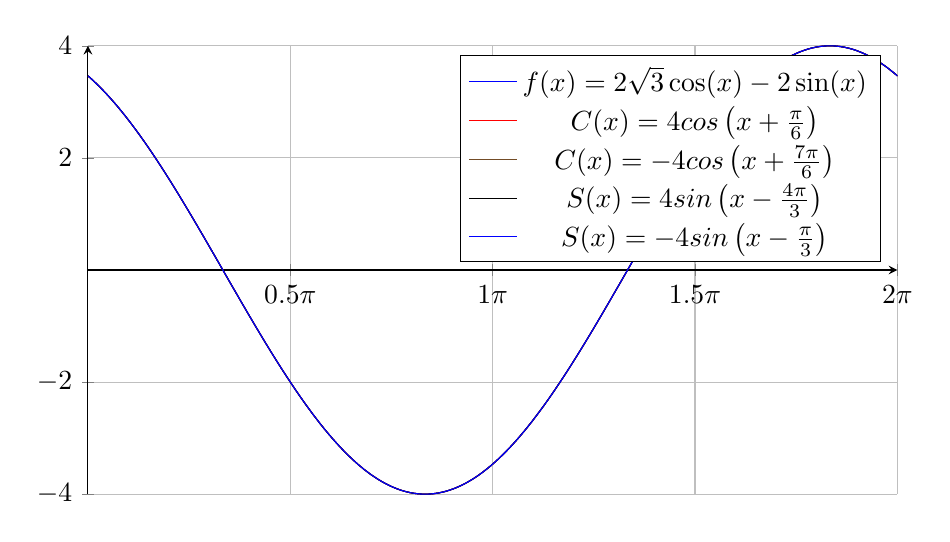
\begin{tikzpicture}
        \begin{axis}
            [
            grid=both,
            axis lines=middle,
            domain=0:2*pi,
            samples=200,
            no marks,
            xticklabels={-2$\pi$,-1.5$\pi$,...$\pi$,2$\pi$},
            xtick={-6.2832,-4.7124,...,6.2832},
            x post scale=1.5
            ]
            \addplot{((2 * sqrt(3)) * cos(deg(x)) - (2 * sin(deg(x))};
            \addlegendentry{$f(x) = 2\sqrt{3}\cos(x) - 2\sin(x)$};
            \addplot {4 * cos(deg(x + (pi / 6)};
            \addlegendentry{$C(x) = 4 cos \left( x + \frac{\pi}{6} \right)$};
            \addplot {-4 * cos(deg(x + ((7 * pi) / 6))};
            \addlegendentry{$C(x) = -4 cos \left( x + \frac{7\pi}{6} \right)$};
            \addplot {4 * sin(deg(x - ((4 * pi) / 3)};
            \addlegendentry{$S(x) = 4sin \left( x - \frac{4\pi}{3} \right)$};
            \addplot {-4 * sin(deg(x - ((pi) / 3))};
            \addlegendentry{$S(x) = -4sin\left( x - \frac{\pi}{3} \right)$};
        \end{axis}
    \end{tikzpicture}
    
    \[C(x) = 4 cos \left( x + \frac{\pi}{6} \right) \]
    \[C(x) = -4 cos \left( x + \frac{7\pi}{6} \right) \]
    \[S(x) = 4sin \left( x - \frac{4\pi}{3} \right) \]
    \[S(x) = -4sin\left( x - \frac{\pi}{3} \right) \]
\end{solution}


\pagebreak


\begin{problem}[35]
    Show that if $f(x) = Asin(\omega x + \alpha) + B$, then $f(x) = Acos(\omega x + \beta) + B$ where $\beta = \alpha - \frac{\pi}{2}$.
\end{problem}

\begin{solution}
    This becomes easy to demonstrate when we look at what $\alpha$ in these functions represents, which is the phase shift. Sine and cosine are identical waves, sine is just shifted to the right by $\frac{\pi}{2}$. So it would stand to reason that when $\beta$ in this instance is just $\alpha - \frac{\pi}{2}$ that you would get two equivalent waves. We can demonstrate this with a plot.
    
    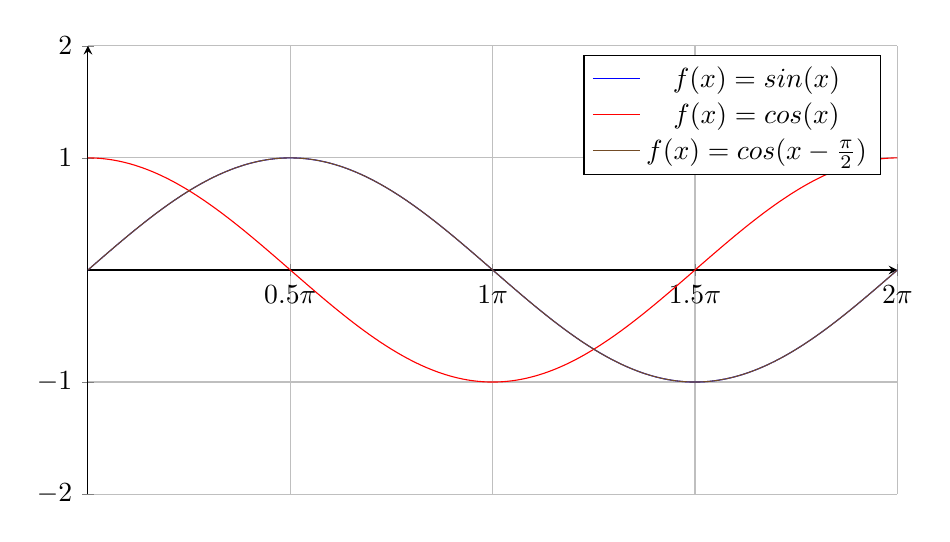
\begin{tikzpicture}
        \begin{axis}
            [
            grid=both,
            axis lines=middle,
            domain=0:2*pi,
            samples=200,
            no marks,
            xticklabels={-2$\pi$,-1.5$\pi$,...$\pi$,2$\pi$},
            xtick={-6.2832,-4.7124,...,6.2832},
            x post scale=1.5,
            ymin = -2,
            ymax = 2
            ]
            \addplot{sin(deg(x))} ;
            \addlegendentry{$f(x) = sin(x)$};
            \addplot {cos(deg(x))};
            \addlegendentry{$f(x) = cos(x)$};
            \addplot {cos(deg(x - (pi / 2)))};
            \addlegendentry{$f(x) = cos(x - \frac{\pi}{2})$};
        \end{axis}
    \end{tikzpicture}
\end{solution}


For exercises 38--40, verify the identity by graphing the right and left hand sides on a calculator.

\begin{problem}[38]
    $sin^2(\theta) + cos^2(\theta) = 1$
\end{problem}

\begin{solution}
    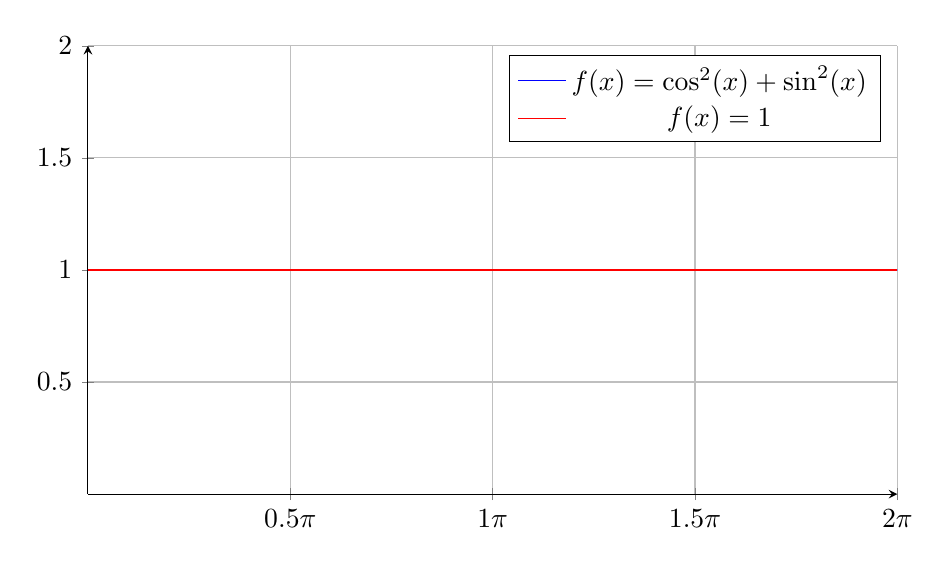
\begin{tikzpicture}
        \begin{axis}
            [
            grid=both,
            axis lines=middle,
            domain=0:2*pi,
            samples=200,
            no marks,
            xticklabels={-2$\pi$,-1.5$\pi$,...$\pi$,2$\pi$},
            xtick={-6.2832,-4.7124,...,6.2832},
            x post scale=1.5,
            ymin = 0,
            ymax = 2
            ]
            \addplot{(cos(x)^2) + (sin(x)^2)} ;
            \addlegendentry{$f(x) = \cos^2(x) + \sin^2(x)$};
            \addplot {1};
            \addlegendentry{$f(x) = 1$};
        \end{axis}
    \end{tikzpicture}
\end{solution}


\pagebreak


\begin{problem}[39]
    $sec^2(\theta) + tan^2(\theta) = 1$
\end{problem}

\begin{solution}
    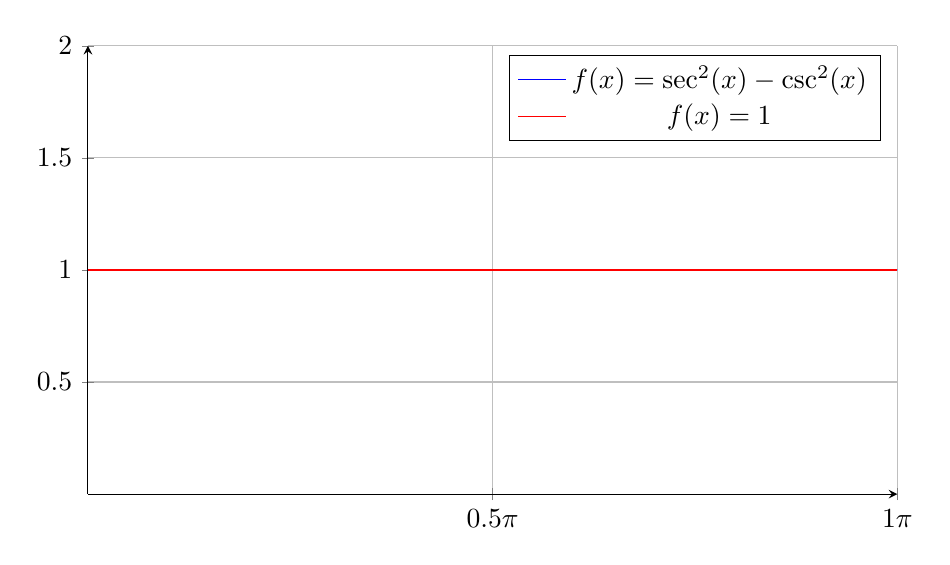
\begin{tikzpicture}
        \begin{axis}
            [
            grid=both,
            axis lines=middle,
            domain=0:pi,
            samples=200,
            no marks,
            xticklabels={-2$\pi$,-1.5$\pi$,...$\pi$,2$\pi$},
            xtick={-6.2832,-4.7124,...,6.2832},
            x post scale=1.5,
            ymin = 0,
            ymax = 2
            ]
            \addplot{(sec(x)^2) - (tan(x)^2)} ;
            \addlegendentry{$f(x) = \sec^2(x) - \csc^2(x)$};
            \addplot {1};
            \addlegendentry{$f(x) = 1$};
        \end{axis}
    \end{tikzpicture}
\end{solution}


\begin{problem}[40]
    $\cos(x) = sin \left( \frac{\pi}{2} - 2 \right)$
\end{problem}

\begin{solution}
    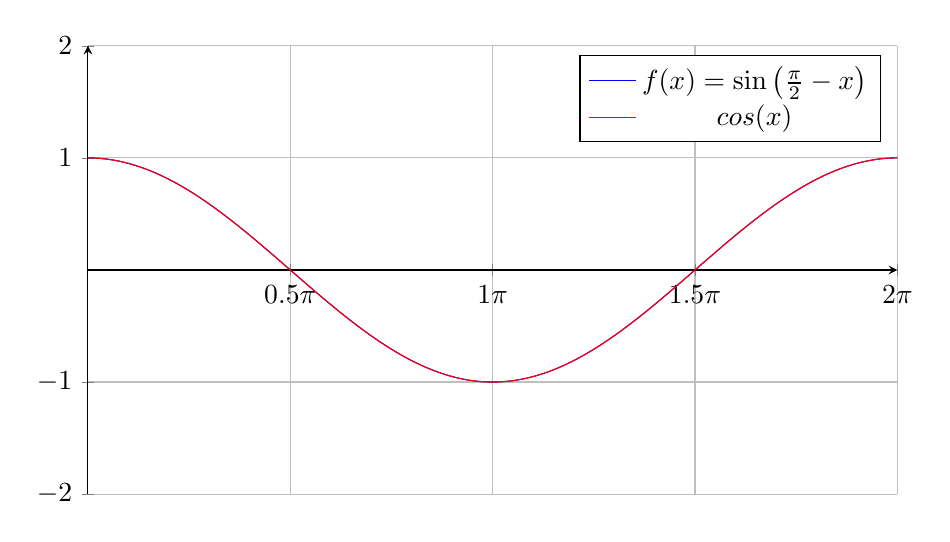
\begin{tikzpicture}
        \begin{axis}
            [
            grid=both,
            axis lines=middle,
            domain=0:2*pi,
            samples=200,
            no marks,
            xticklabels={-2$\pi$,-1.5$\pi$,...$\pi$,2$\pi$},
            xtick={-6.2832,-4.7124,...,6.2832},
            x post scale=1.5,
            ymin = -2,
            ymax = 2
            ]
            \addplot{sin(deg((pi/2)-x)))} ;
            \addlegendentry{$f(x) = \sin \left( \frac{\pi}{2} - x \right)$};
            \addplot {cos(deg(x))};
            \addlegendentry{$cos(x)$};
        \end{axis}
    \end{tikzpicture}
\end{solution}


\pagebreak


In exercises 44--50, graph the functions and discuss the given questions.

\begin{problem}[44]
    $f(x) = \cos(3x) + sin(x)$. 
    
    Is this function periodic? If so, what is the period?
\end{problem}

\begin{solution}
    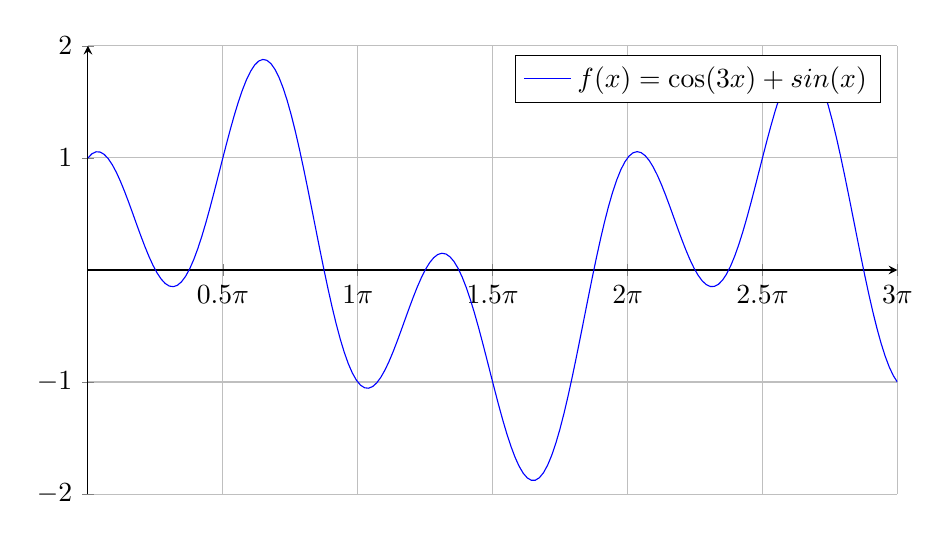
\begin{tikzpicture}
        \begin{axis}
            [
            grid=both,
            axis lines=middle,
            domain=0:3*pi,
            samples=200,
            no marks,
            xticklabels={-2$\pi$,-1.5$\pi$,...$\pi$,2$\pi$, 2.5$\pi$, 3$\pi$},
            xtick={-6.2832,-4.7124,...,6.2832, 7.853982, 9.424778},
            x post scale=1.5,
            ymin = -2,
            ymax = 2
            ]
            \addplot {(cos(deg(3*x))) + (sin(deg(x)))};
            \addlegendentry{$f(x) = \cos(3x) + sin(x)$};
        \end{axis}
    \end{tikzpicture}
    
    This function is periodic even if it doesn't appear to be at first glance. Going off of the plot alone the period seems to be right around $2\pi$ as normal. Looking at the function we know we're combining two periodic functions. $cos(3x)$ is going to repeat way faster than normal, whereas $sin(x)$ will have a standard period of $2\pi$. So why does the overall function have a period of $2\pi$? We can calculate it to find out. Let's get the period of our sine and cosine individually first.
    
    \begin{align}
        3x_{cos} = 2\pi && x_{sin} = 2\pi \\
        x_{cos} = \frac{2\pi}{3}
    \end{align}
    
    The period of $f(x)$ then is the least common multiple of $x_{cos}$ and $x_{sin}$. Upon inspection we can see that the L.C.M is $2\pi$. 
\end{solution}


\pagebreak


\begin{problem}[45]
    $f(x) = \frac{\sin(x)}{x}$
    
    What appears to be the horizontal asymptote of the graph?
\end{problem}

\begin{solution}
    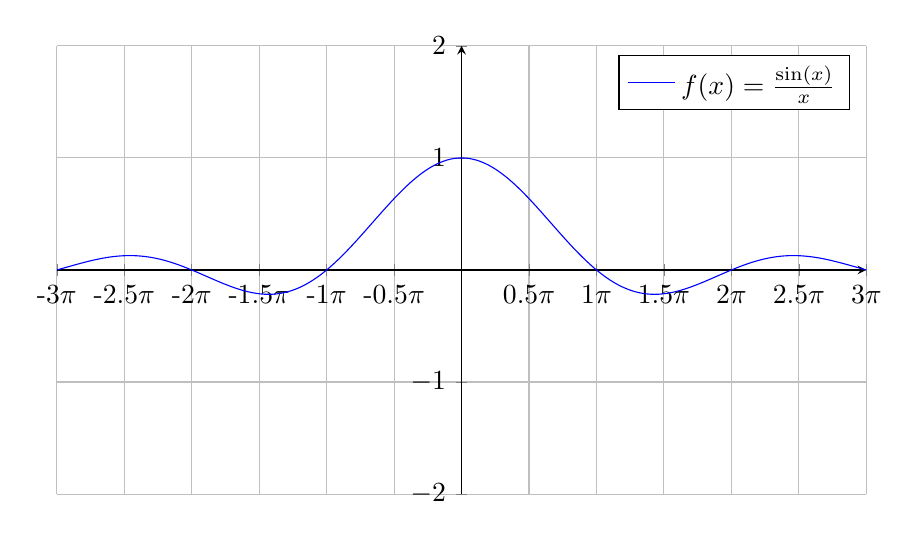
\begin{tikzpicture}
        \begin{axis}
            [
            grid=both,
            axis lines=middle,
            domain=-3*pi:3*pi,
            samples=200,
            no marks,
            xticklabels={-3$\pi$, -2.5$\pi$, -2$\pi$,-1.5$\pi$,...$\pi$,2$\pi$, 2.5$\pi$, 3$\pi$},
            xtick={-9.424778, -7.853982, -6.2832,-4.7124,...,6.2832, 7.853982, 9.424778},
            x post scale=1.5,
            ymin = -2,
            ymax = 2
            ]
            \addplot {(sin(deg(x))) / x};
            \addlegendentry{$f(x) = \frac{\sin(x)}{x}$};
        \end{axis}
    \end{tikzpicture}
    
    The horizontal asymptote appears to be at f(x) = 0. This makes sense as due to x being in the denominator it can never be zero, and as x grows the fraction will simply get closer and closer to zero as it reaches infinity in either direction.
\end{solution}


\begin{problem}[46]
    $f(x) = x \cdot sin(x)$. 
    
    Graph $y = \pm x$ on the same set of axes and describe the behavior of $f$. 
\end{problem}

\begin{solution}
    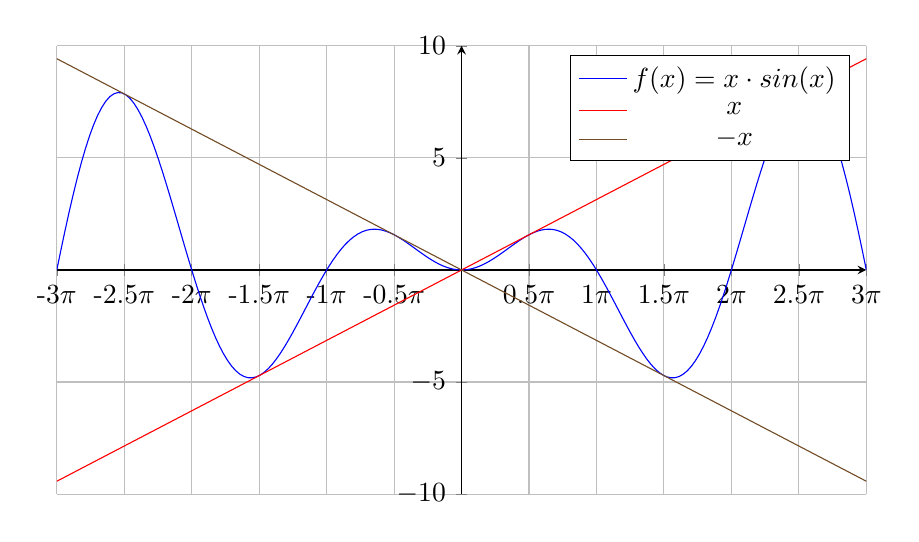
\begin{tikzpicture}
        \begin{axis}
            [
            grid=both,
            axis lines=middle,
            domain=-3*pi:3*pi,
            samples=200,
            no marks,
            xticklabels={-3$\pi$, -2.5$\pi$, -2$\pi$,-1.5$\pi$,...$\pi$,2$\pi$, 2.5$\pi$, 3$\pi$},
            xtick={-9.424778, -7.853982, -6.2832,-4.7124,...,6.2832, 7.853982, 9.424778},
            x post scale=1.5,
            ymin = -10,
            ymax = 10
            ]
            \addplot {(x * sin(deg(x)))};
            \addlegendentry{$f(x) = x \cdot sin(x)$};
            \addplot {x};
            \addlegendentry{$x$};
            \addplot {-x};
            \addlegendentry{$-x$};
        \end{axis}
    \end{tikzpicture}
    
    So, what's happening here? So, first the obvious. As x grows the amplitude also grows. Also, the local maximums and minimums match up precisely with $y = \pm x$. This relationship will continue to hold true as $x$ reaches infinity in either direction. $f(x)$ will, in a sense, never actually leave the boundaries set by $y = \pm x$.
\end{solution}


\pagebreak


\begin{problem}[47]
    $f(x) = sin \left( \frac{1}{x} \right)$
    
    What's happening as $x \rightarrow 0$?
\end{problem}

\begin{solution}
    
   What's happening here is that as x approaches zero the periodicity of the function gets bigger and bigger. This means it completes cycles faster and faster as we get closer to zero. I would describe the graph as violently oscillating between 1 and -1 at a speed that impossible for me to comprehend. The software I use for plots doesn't handle functions like this particularly well due to a limitation of given points. As such I used the software desmos which handles continuous graphs better.
    
    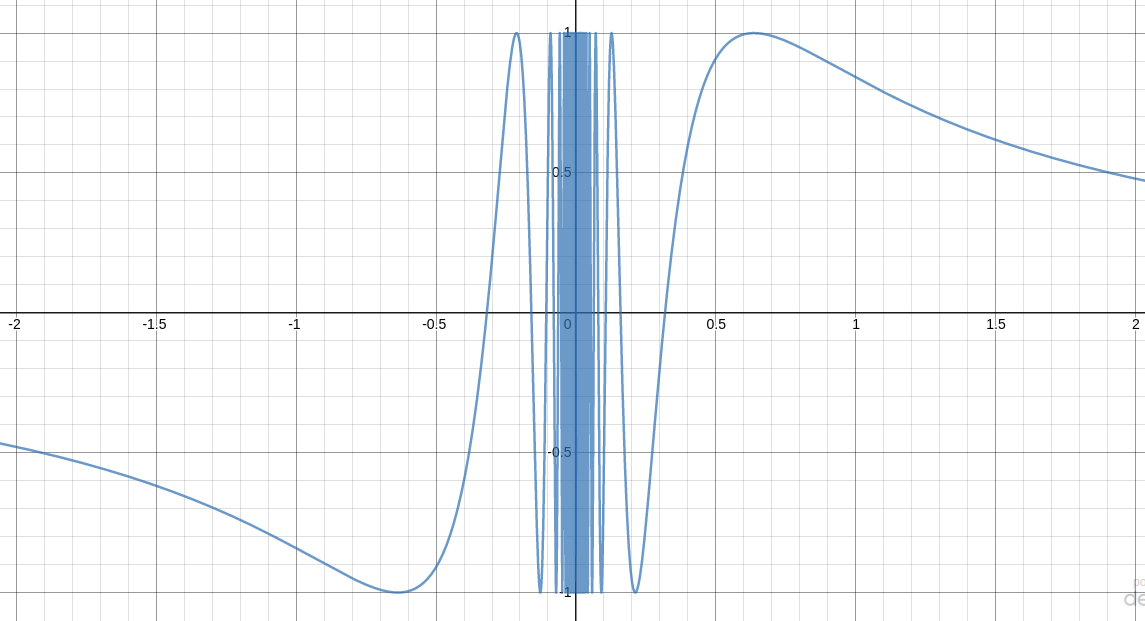
\includegraphics[width=6in,scale=1.0]{images/pr_47.png}
\end{solution}


\begin{problem}[48]
    $f(x) = x - tan(x)$
    
    Graph $y = x$ on the same set of axes and describe the behavior of $f$.
    
\end{problem}

\begin{solution}
    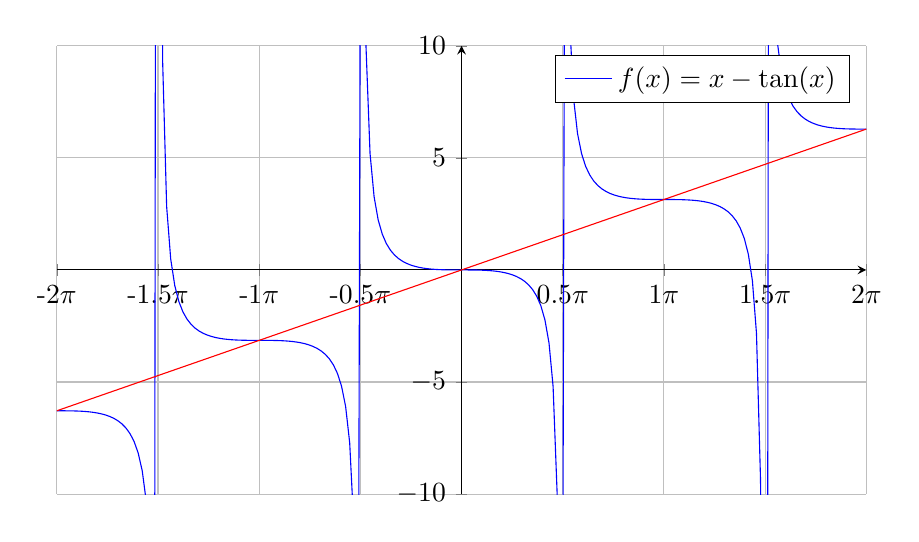
\begin{tikzpicture}
        \begin{axis}
            [
            grid=both,
            axis lines=middle,
            domain=-2*pi:2*pi,
            samples=200,
            no marks,
            xticklabels={-3$\pi$, -2.5$\pi$, -2$\pi$,-1.5$\pi$,...$\pi$,2$\pi$, 2.5$\pi$, 3$\pi$},
            xtick={-9.424778, -7.853982, -6.2832,-4.7124,...,6.2832, 7.853982, 9.424778},
            x post scale=1.5,
            ymin = -10,
            ymax = 10
            ]
            \addplot {(x - tan(deg(x)))};
            \addlegendentry{$f(x) = x - \tan(x)$};
            \addplot{x};
        \end{axis}
    \end{tikzpicture}
    
    So, what's happening here is that the center point of each tangent period is increasing/decreasing alongside the $y=x$ function. Normally those center points are all right at $y=0$. 
\end{solution}


\begin{problem}[49]
    $f(x) = e^{-0.1x} (\cos(2x) + sin(2x))$
    
    Graph $y = \pm e^{-0.1x}$ and describe the behavior of $f$.
\end{problem}

\begin{solution}
    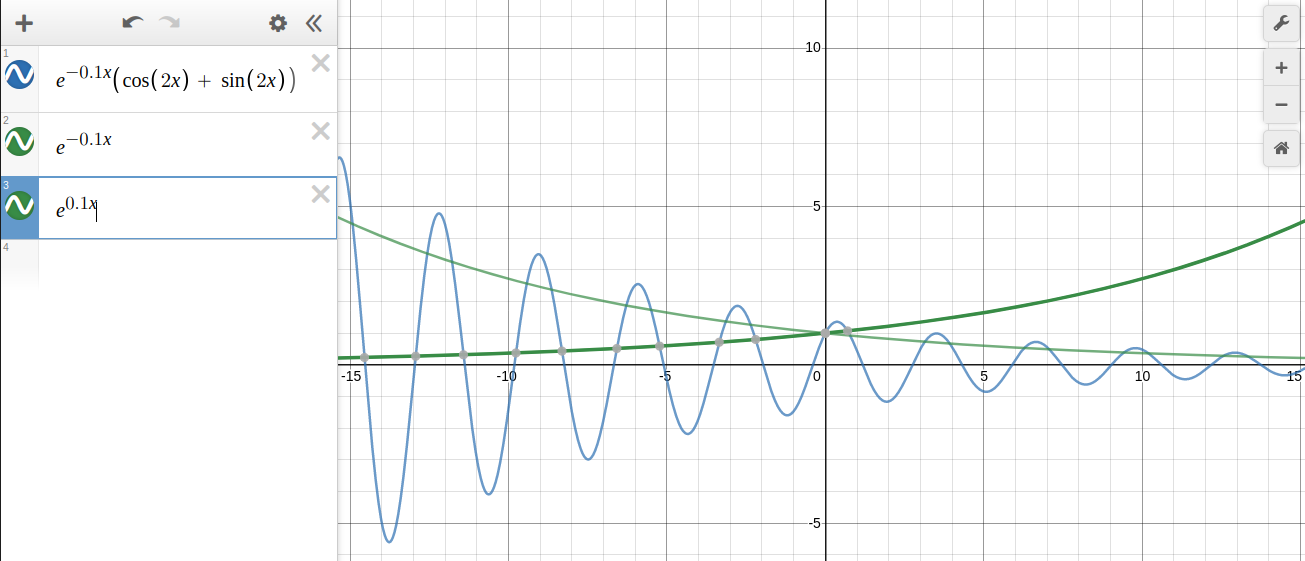
\includegraphics[width=6in,scale=1.0]{images/pr_49.png}
    
    $f(x)$ intersects twice with $e^{-0.1x}$ near its local maximums consistently along the entire domain of \\ $(-\infty, \infty)$.
\end{solution}


\begin{problem}[50]
    $f(x) = e^{-0.1x} (\cos(2x) + 2sin(x))$
    
    Graph $y = \pm e^{-0.1x}$ and describe the behavior of $f$.
\end{problem}

\begin{solution}
    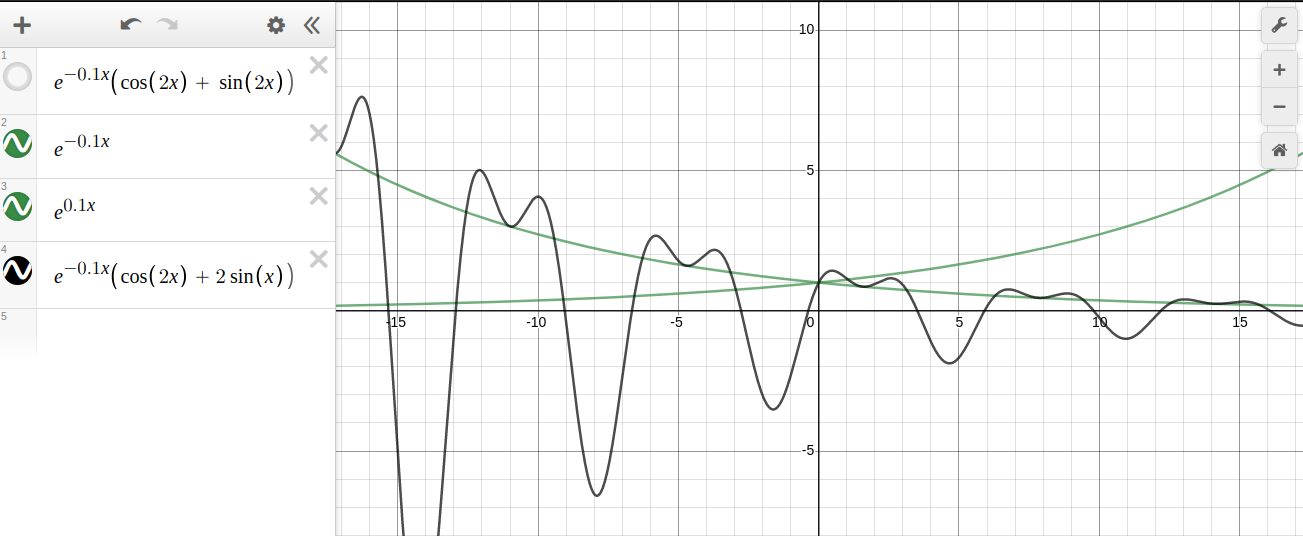
\includegraphics[width=6in,scale=1.0]{images/pr_50.png}
    
    So, this may not be the best description but I would say that with every "period" of the graph you have bimodal humps that ride along $e^{-0.1x}$ as $f(x)$ goes from $-\infty \rightarrow 0$. This behavior continues along the entire domain but the amplitude goes down as x reaches $\infty$. 
\end{solution}
\end{document}